Aquí pueden encontrarse gráficos adicionales sobre los métodos empleados
en este trabajo.

\subsubsection{Ley de Zipf}
\label{appendix-plots-zipf-law}
\begin{figure}[h!]
    \centering
    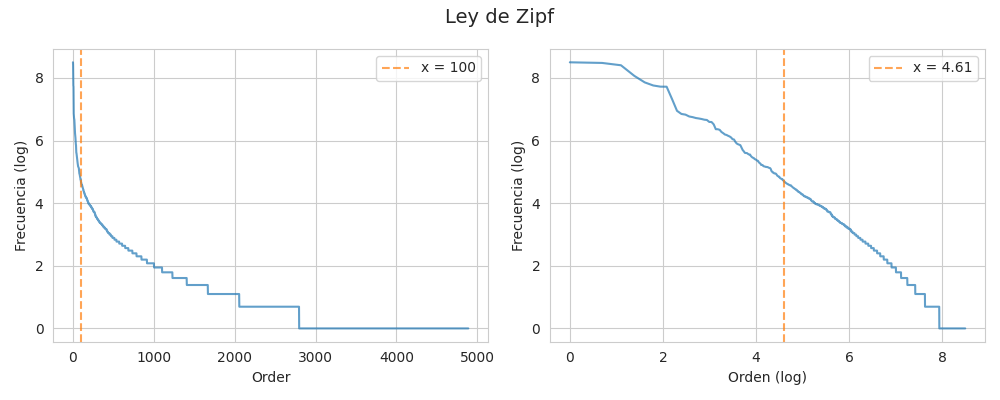
\includegraphics[scale=0.4]{../visualizations/ley_de_zipf.png}
    \caption{Contraste entre la frecuencia absoluta de cada palabra (en logaritmo)
    y el \textit{ranking} de esa palabra según su frecuencia. El gráfico de la
    derecha exhibe el orden natural de cada palabra y el de la izquierda, su logaritmo.
    En ambos casos, la línea punteada naranja indica el umbral
    para considerar \textit{stopword} a una palabra.}
    \label{fig-zipf-law}
\end{figure}